
\documentclass[a4paper]{sbgames}               % final
%\usepackage[scaled=.92]{helvet}
\usepackage{times}
\usepackage{graphicx}

%% use this for zero \parindent and non-zero \parskip, intelligently.
\usepackage{parskip}

%% the 'caption' package provides a nicer-looking replacement
\usepackage[labelfont=bf,textfont=it]{caption}
\usepackage[latin1]{inputenc}

\usepackage{url}

\newcommand{\ppse}{Proj48534}
\newcommand{\hoverkill}{HK48534}

%% Paper title.
\title{\ppse{} - A Peer-to-Peer Support for Multiplayer Games}

\author{JEMS Manuscript Number 48534}
\contactinfo{48534@JEMS}
% %% Author and Affiliation (multiple authors). Use: and between authors
% \author{Felipe J. Vilanova, Carlos Eduardo B. Bezerra , Marcos R. Crippa, F�bio R. Cecin, Cl�udio F. R. Geyer\\
%           Universidade Federal do Rio Grande do Sul\\
%           Bento Gon�alves, 9500\\
%           Porto Alegre, RS, Brazil\\
%           +55 (51) 3316 0000
% }
% \contactinfo{\{fjvilanova, carlos.bezerra, mrcrippa, fcecin, geyer\}inf.ufrgs.br}


%% Keywords that describe your work.
\keywords{Peer-to-peer, Descentralization, Scalability, Multiplayer Games, Hybrid Topologies, Instanced Game, Distributed Systems}

%% Start of the paper
% Attention: As you need to insert EPS images in Postscript, 
% you need to insert PDF images into PDFs. 
% In the text, extensions cancbe omitted (latex use .eps, pdflatex get .pdf) 
% To convert them: epstopdf myimage.eps
\begin{document}

%\teaser{
%  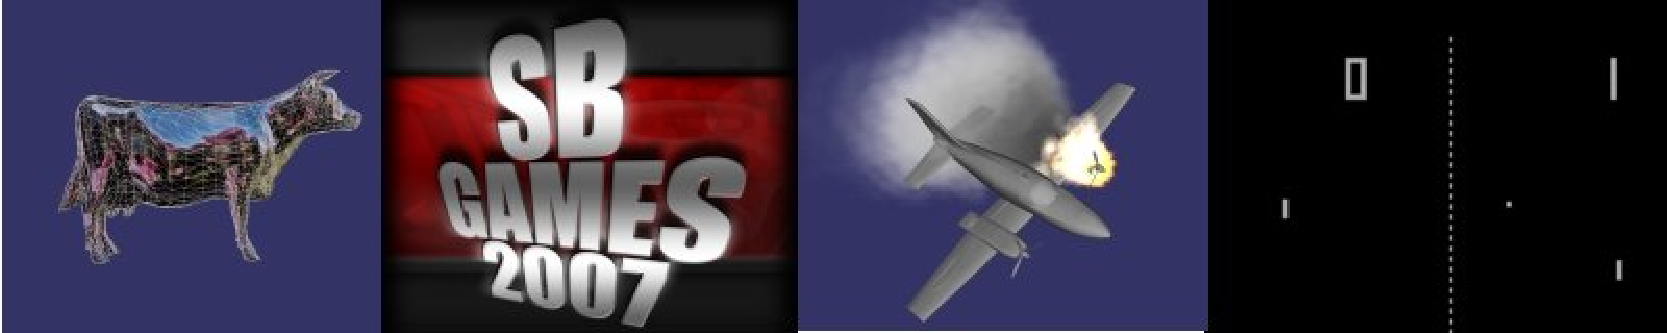
\includegraphics[width=\linewidth]{sample.pdf}
%  \caption{Optional image}
%}

%% The ``\maketitle'' command must be the first command after the
%% ``\begin{document}'' command. It prepares and prints the title block.

\maketitle

%% Abstract section.

\begin{abstract}

  The successful commercial MMOGs, at the moment, are implemented using some variant of the client-server model. This model offers simple design, good security and fast detection and treatment of cheating. However, it lacks scalability. The cost of maintaining the server becomes excessive with the increased number of customers. One approach to deal with this situation is distributing the MMOG simulation. The changes in the virtual world of the game would be processed by the machines of the clients, without interference from the server. This distribution can be achieved using the peer-to-peer model. In this paper, we describe a network engine, called \ppse{}, which supports partially decentralized MMOGs, ensuring scalability and flexibility, while guaranteeing the basic properties of a client-server model, such as security and consistency. We first examine in more details the existent distributed models. After that, we discuss about the \ppse{} project and its characteristics. Finally we present a simulation of the architecture in comparison with the traditional client-server model.

\end{abstract}

%% The ``\keywordlist'' command prints out the keywords.
\keywordlist
\contactlist

\section{Introduction}
\label{sec:intro}

Multiplayer games are a very popular game genre, due to their highly interactive nature. Among those games, a class that is growing in popularity is MMOGs (Massively Multiplayer Online Games). MMOGs are real-time multiplayer games played through the Internet, where a great number of players (usually thousands) play within a persistent-state virtual world. Successful examples include EverQuest \cite{everquest} and World of Warcraft \cite{worldofwarcraft}.

The most common network model used in MMOGs is client-server. In this model, the client only sends its data to the server-side (that can operate on a single machine, a cluster or a grid) and receives frequent updates from the server. The server process all the data from the clients, and broadcasts all the results that occur on the virtual world back to them. Some advantages of this model are: being simple in design; cheating can be efficiently detect and stopped; retaining control over access to the game; and being a predictable model.

The main disadvantage of the client-server model is the lack of scalability. The cost of maintaining the server-side becomes excessive with the increase in the number of clients. When talking about commercial games, the usual approach is to continuously expand the number of machines on the server-side. That is a reasonable solution, however it is not suitable for projects on a budget such as those from small companies or research groups. 

One way of dealing with the above problem is to fully or partially distribute the MMOG simulation. All the changes on the game world would be registered and dealt within the client-side, with no interference of the server-side. Security and world state consistence are issues on that model, because there isn't a point where the changes in the virtual world can be evaluated and considered legal or illegal. The main challenge of our project is thus to provide a partially decentralized support model for MMOGs, while retaining the basic properties of the client-server model such as security, consistency and scalability \cite{schiele2007rpp}.

In this paper a hybrid model is proposed, combining the security and consistency of the client-server model with the scalability and flexibility of the distributed model. In sections \ref{sec:c-smodel} and \ref{sec:p2pmodel} we discuss the client-server and peer-to-peer models. The \ppse{} %(acronym in portuguese for ``P2P for Entertainment Software'') 
architecture is explained in section \ref{sec:p2pse}. Section \ref{sec:simulations} presents the simulations we made to compare client-server and peer-to-peer models. Section \ref{sec:conclusion} presents conclusions on the topic.

\section{Client-server model}
\label{sec:c-smodel}

The client-server paradigm is undoubtedly the most currently used in the implementation of Internet real-time multiplayer games. Commercial examples of these games include Doom \cite{doom}, Quake \cite{quake} and Counter-Strike \cite{counterstrike}, all them 3D real time action games. In any client-server game, massively multiplayer or not, the players interact with the environment and with other players through a client program. Each client has a network connection only with the server. The server is responsible for receiving the information from each client and passing updates to the other clients. There are several different ways the communication protocol between the client and the server can be implemented: some of them provide more security, while others provide efficiency.

Regardless of the technique used, the server is responsible for maintaining the game state up-to-date. Since the game is a real time simulation, it is necessary for the state of the game to be frequently recalculated. In general, the server is configured to update its state in a fixed and relatively small frequency, and to periodically send update messages to all clients. Due to that, the server must have great processing power (CPU and, indirectly, memory) and enough bandwidth (network).

A distributed game can use the centralized simulation to accommodate thousands of simultaneous clients. In practice, however, it can be difficult to have in a single machine all the processing power required to perform the simulation in real time. One solution to this problem, commonly used in commercial MMOGs such as EverQuest and PlanetSide \cite{planetside}, is to divide the virtual world and simulate each division in an individual machine as, for example, a particular computer in a cluster of computers. But even using the clusters to mitigate the problem of the server processing cost, the problem of network consumption still remains. The MMOG server, a single machine or a cluster, will need an Internet connection with low latency and very high bandwidth.


\section{Peer-to-peer model}
\label{sec:p2pmodel}

There is a growing interest in research and development of peer-to-peer architectures for MMOGs. The models proposed seek decentralization as a way of increasing scalability and reducing dependency on nodes in trusted areas. Other benefits include the elimination of central points of failure, as well as the increase of responsiveness.

The Communications Architecture for Massive Multiplayer Games, proposed by \cite{fiedler2002cam}, was the first architecture to address the scalability problem by proposing a solution based on the publisher-subscriber paradigm. In this paradigm, the virtual world is divided into smaller pieces, usually called "cells", and each participant can choose to sign (or participate) in only a few cells. Thus, each subscriber of a cell only needs to exchange update messages with subscribers of the same cell. These architectures also deal with other fundamental problems, such as the problem of responsiveness to commands generated by each participant.

There are other proposals that do not address the cheating problem, such as Hydra \cite{chan2007hmm}, that focuses on guaranteeing the consistency in the messages committed when nodes fail; and Mediator \cite{fan2007mdf}, which addresses the scalability and performance problems by proposing a solution based on a super-peer network and a reward scheme: peers that contribute more can use more resources.  

It can be noted that recent proposals for MMOG support based on peer-to-peer overlays are becoming more aware of issues in actually deploying a peer-to-peer MMOG on the Internet, as they show more concern about peer-to-peer problems, like hostile service providers and bandwidth limitations, for instance. There are many pure peer-to-peer and hybrid model proposals. However, some of these proposals don't offer any kind of deterrent mechanism against cheating players, which is an essential feature for implementing an online massively distributed and persistent-state game. In the next section we will show how our model offers scalability and also cheat-resistance so that its commercial application is viable.



\section{\ppse{} project}
\label{sec:p2pse}

The \ppse{} project is a distributed simulation model, and also a library (in reality, a stack of C/C++ libraries) that implements the instanced game model, which will be described in section \ref{sec:p2pse:instanced}. The instanced game model is the price to pay for a simple approach in unifying security, consistency and scalability in a decentralized MMOG. The objective is to drastically reduce the processing and communication cost in the server-side.

\subsection{The Instanced Game Model}
\label{sec:p2pse:instanced}

Several MMOGs, like PlanetSide and World of Warcraft, offer to the player the illusion of one or several large and contiguous virtual spaces where all the gaming takes place. Those spaces are divided in segments, and each server machine or group of server machines is responsible for one segment. A warping system is necessary to tie all segments together, allowing the player to move from one space to the other transparently.

\begin{figure}[h] 
  \centering 
  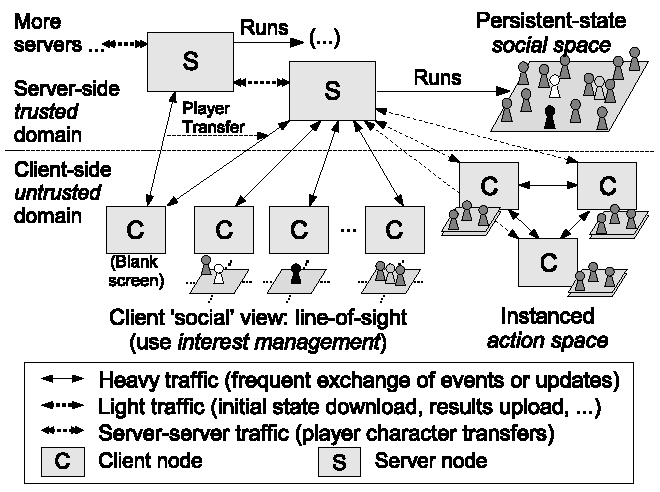
\includegraphics[width=1.0\linewidth]{images/instanced.pdf}
 \caption{The instanced `social vs. action' MMOG} 
 \label{fig:instanced} 
\end{figure}

The game Guild Wars introduced a new game model, which will be referenced to as the instanced game model \cite{cecin2006pps}. There are two virtual spaces on Guild Wars: the social space and the action space. The first kind is a medium-sized virtual space where a significant number of players can socialize, trade virtual goods and organize game sessions. Because of the nature of this space, low consistency requirements are necessary. Game sessions happen on the action space, which is a small-sized virtual space where a small number of players gather to play a game session. Higher consistency requirements are necessary on that space because of its fast and dynamic nature.

The relationship between the two spaces is as follows. When a game session ends, the players involved in it return to the social space. All the traits of the characters (e.g. virtual world money, experience points and statistics) are updated with new information from the session. The social space is designed as a contiguous world, as mentioned in the beginning of this section. The action spaces are created dynamically to support temporary game sessions with a small number of players. This space is destroyed after the session ends.

Guild Wars, as far as we can tell, follows the client-server model. Our proposal, which is illustrated in Figure \ref{fig:instanced}, is to use the instanced game model with a hybrid network architecture model. Since the interactions on the social space (chatting, trading) don't require high consistency, and there is a necessity for validation of who can play (game accounts, passwords), the server-side will be responsible for coordinating this part of the game. So even a server-side with modest processing capacity and network bandwidth could manage the social space if game quality is scaled down accordingly, for instance by sending less frequent updates to clients. The game sessions would be processed only on the client-side machines, avoiding unnecessary processing and communication cost on the server-side. The clients would form groups, wich would operate within a peer-to-peer dynamics.

\subsection{\ppse{} architecture}
\label{sec:p2pse:arch}

\begin{figure}[h]
  \centering 
  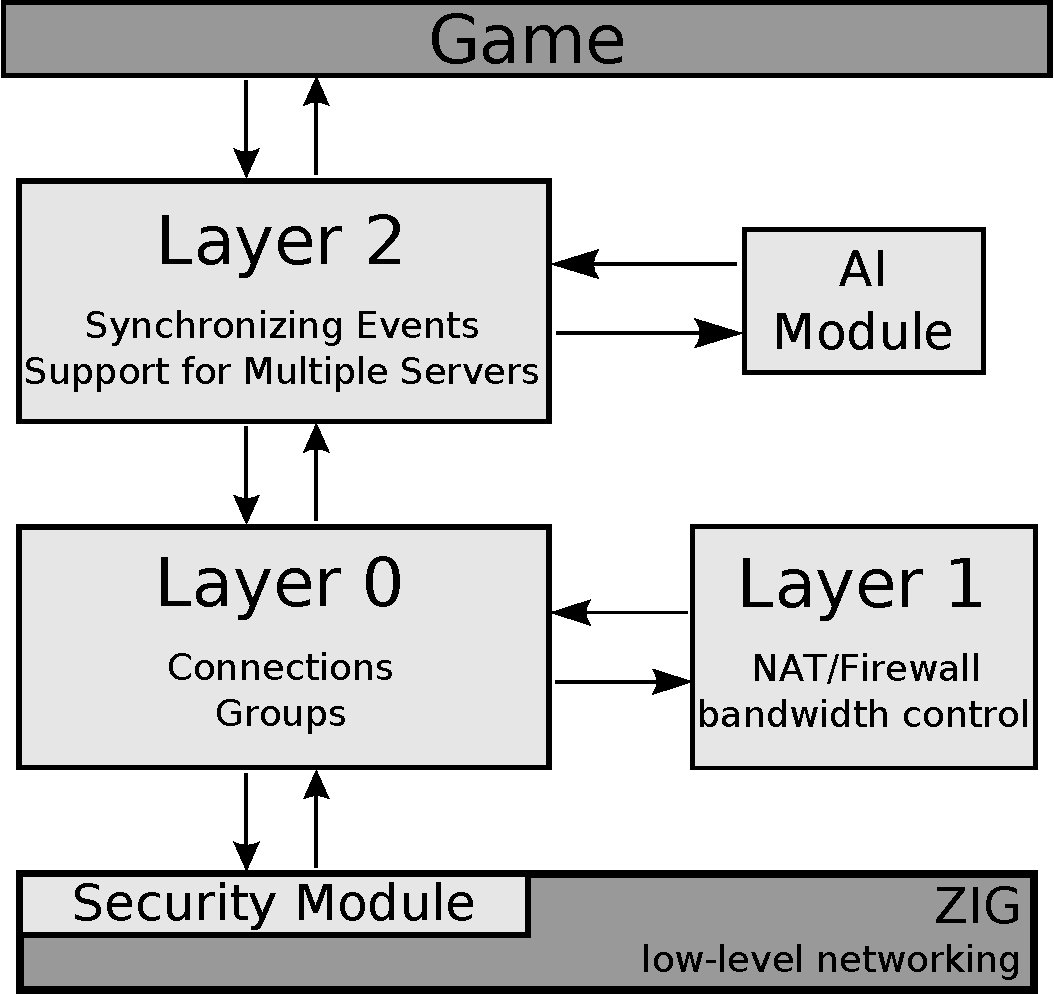
\includegraphics[width=1.0\linewidth]{images/p2pse.pdf}
 \caption{\ppse{} Architecture} 
 \label{fig:p2pse} 
\end{figure}

The functionality promised by our network engine is delivered by a set of libraries. Those libraries are organized in layers, as shown in Figure \ref{fig:p2pse}. The next sections describe the implementation of the three layers, followed by an overview of security and artificial intelligence (AI) techniques which are employed.

\subsubsection{Layer 0}
\label{sec:p2pse:arch:l0}

The first layer in the \ppse{} architecture is responsible for forming the mesh of point-to-point connections. The clients' connections with the servers and with other clients are established and managed in this layer. The basic network functions for connection establishment, such as socket creation, connection and packet sending and receiving, are given by a low-level API provided by the ZIG library \cite{zige} which basically implements a protocol that resembles SCTP \cite{stewart2000sct} over UDP.

The Layer 0 server is responsible for managing connections with all clients. Naturally, it maintains a list of all clients that are connected to it along with a logical communication endpoint object for each client. When started, the server spawns a socialization space called the social space object. The clients that are not in an action space are bound to the social space - or to the ``limbo'', when in transit from one space to the other. All communication between clients that are in the social space is intermediated by the server.

The server can create new empty groups in order to instantiate new action spaces, or destroy such existing groups and their corresponding spaces. In the action spaces all the clients communicate directly, which requires them to already have the ability to send UDP packets to one another. The entry of a client into a group is managed by the server in the following manner:

\begin{enumerate}
\item The server sends a synchronization message to the new member and to all the other members informing them to which clients they must be connected in order to enter (or stay) in the group. The server sends a list with all the members of the group;
\item All members then try to establish connections to every other member in the recently received member list, or just keep the connection, if it has already been established (the ZIG library supports simultaneous bidirectional connections through the same socket);
\item When a client is entering a group, but still has not finished the process, it belongs to the ``limbo'';
\item As soon as the new member establishes connections to the other clients, the server excludes it from the limbo and inserts it in the member list of the group;
\item When a client is removed from the group, all connections to the other clients are interrupted and it returns to the social space;
\item If a client, for any reason, loses its connection to the server, it is removed from the group;
\item When a client enters or leaves a group, the server sends to the others  an up-to-date member list.
\end{enumerate}

The groups provide to the clients message exchanging functionalities, such as broadcast and unicast. The connections between the group members are represented by peers. The clients, when in groups, will keep a list of peers, what is equivalent to the client list of the server. With this list, the clients in that group manage their connections between one another.

Layer 0 is also responsible for the timeout control of the connections. Keep-alive dummy messages are sent regularly in order to maintain all connections active. If, after an interval of time specified by the application, no messages from a host have arrived, the connection to that host is closed.

The communication between the layer 0 and the ZIG library is done with a listener. This listener is implemented in layer 0 and receives ZIG callbacks to indicate the occurrence of events such as connections, disconnections and receiving of messages. The communication between the upper layers of the \ppse{} library and layer 0 is made through service calls. Layer 0 returns callbacks to the upper layers in response to these service calls.


\subsubsection{Layer 1}
\label{sec:p2pse:arch:l1}

Layer 1 of the \ppse{} architecture is responsible for handling connection-related problems between the peers within a group. This layer will ensure that all peers are able to send and receive messages from each other.

We see two main problems that can cause a connection failure between two peers: NAT/Firewall block and bandwidth insufficiency. When the Layer 0 indicates that a message must be send from one peer to another, Layer 1 must verify if there is a direct connection between the peers. If this connection doesn't exist, an alternative path must be discovered, using intermediate peers. After the path is discovered, the proper routing of the message can take place.

Among all peers within a group there are different bandwidth capabilities. It is very likely to occur a situation where a peer doesn't have enough upload bandwidth to deal with the number of messages that it has to send. Layer 1 will identify such situation and, instead of sending the messages directly to the  destinations, send them to a peer with good upload bandwidth capability, holding him responsible to send the message. 

\subsubsection{Layer 2}
\label{sec:p2pse:arch:l2}

The upper layer of the \ppse{} implementation is responsible for guaranteeing the simulation consistency on action spaces, providing support for multiple servers and exposing all of the implementation's functions to the game programmer. Due to the simulation of action spaces being executed asynchronously in each peer, there is no intrinsic guarantee of consistency. To partially address that, Layer 2 introduces the role of the super-peer, which is a special peer responsible for receiving, ordering and redistributing some of the game events such as updating player scores and picking up the flag in a capture-the-flag action game, for instance. To avoid overloading the super-peer, position updates or player movement requests (depending on the game's protocol design) are to be sent directly from each peer to every other peer using the unicast full-mesh provided by the lower layers. Not only position updates, but any other frequent, delay-sensitive and weakly-coupled message type should also be sent peer-to-peer. 

Depending on the game, the resulting conflicts from a lack of centralized timestamping of movement and similar events, whenever they ensue, can be either handled by each peer individually or left for the super-peer to detect it and issue a special correction message later, as the BZFlag protocol does \cite{pellegrino2003bra}. Local corrections are an option if each peer is authoritative over its own avatar's position and if it broadcasts position updates for its own avatar. For instance, if a peer's local avatar overlaps with a remote peer's, the local avatar can push its own avatar out of that position. The remote avatar will do the same. The only issue is ensuring that the correction step won't make both peers try to resolve the situation by unstucking their avatars to the same spot again. This local conflict resolution is what we are currently employing in our capture-the-flag action prototype, \hoverkill\ [reference blinded].%Hoverkill \cite{hoverkill}. 

Besides ordering and distributing some of the events, the super-peer is responsible for the communication of the peer-to-peer action group with the server. The super-peer is the one that reports gameplay results back to the server, whenever necessary.

Layer 2 also introduces support for multiple game servers (Figure \ref{fig:multiserver}) in the API. The idea is that players can choose their server from a list of servers. Each server will typically host a single social space and when that is full (server capacity is reached) players can connect to other social spaces in other servers. To tie all of the players scattered on different servers together, there is a master server to which all servers are connected. Whenever a player connects to a server and authenticates, his player account is downloaded from the master server to that game server. When the client drops from the game server, his account is uploaded back to the master server. There is a simple Yellow Pages Server proxy that can be used by clients to query the master server for the currently available game servers.

\begin{figure}[h]
  \centering 
  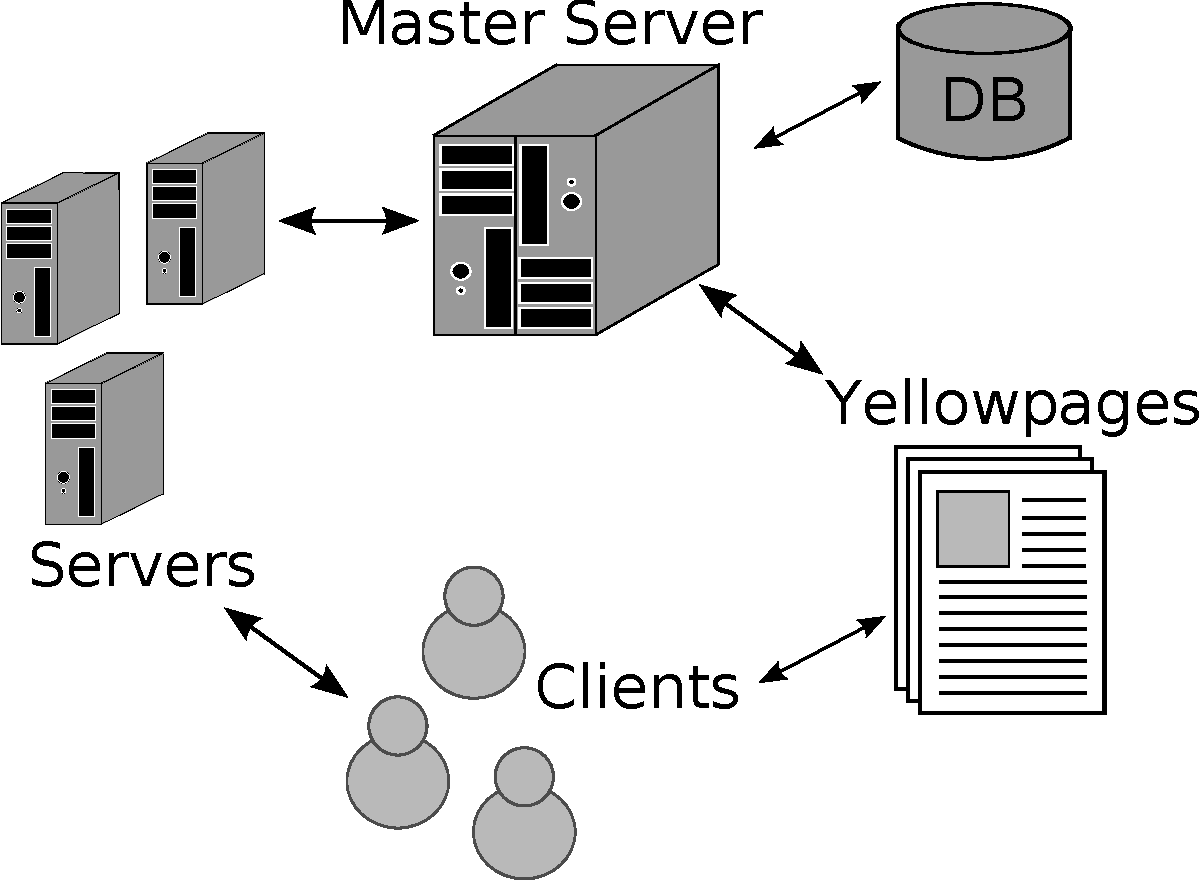
\includegraphics[width=1.0\linewidth]{images/multiserver.pdf}
 \caption{Multiple Servers Support} 
 \label{fig:multiserver} 
\end{figure}

The social space support provided by Layer 2 is a simple client-server API. Any interest management \cite{morse1996iml} in the social space is currently left for the application to implement. We are planning to add something akin to OpenTNL ghosting \cite{opentnl} into the API which would allow the game programmers to optimize the social space more easily. Another idea is to implement a peer-to-peer mesh for social spaces, but that one would have to be scalable (no full-mesh possible). Since we are aiming at a simple solution, the use of probabilistic broadcast for position updates on the social space is being considered, leaving timestamping and distribution of more infrequent events for the server.

\subsubsection{Artificial Intelligence Module}
\label{sec:p2pse:arch:ai}

In the previous section, we revealed that we encourage peers in an action space to send authoritative position updates, among other events that might have low-latency requirements and a low probability of having their order of execution affecting the resulting game states too much (weakly-consistent events). This opens up the possibility of cheating.

In this project we tried a somewhat unique approach [reference blinded]%\cite{gaspareto2008nna}
. Since most events would be still centralized at the super-peer and most action games have one-per-client avatar position updates as their latency, consistency and bandwidth bottlenecks, we just left peers with total control over their positions and with the responsibility for sending them directly to other peers in a broadcast fashion. This optimizes for consistency and latency, and doesn't create a bandwidth bottleneck at the super-peer. On top of that, we tried AI-based detection of unusual patterns over streams of position updates coming from each peer. The approach used for cheat detection was focused on the data packets being transferred during the game sessions - both in the transmitters and receptors - and how they are used during the functioning of the system. Only packets relevant to the cheat being investigated are considered.

The cheat detection module is implemented in an independent way and works as an attachment to \ppse{}, which, with a parameter passage protocol, informs the set of data received from a player and returns a correspondent ``fraud index'', that tries to quantify the cheating that the player is assumed to have performed in the analyzed period.

The adopted approach was to consider only movement data as input to the cheat detection module. Although this might seem to be too few information, it is based on movement that  malicious players perform great part of their cheating. For example, one could try to move at a speed higher than the maximum speed allowed in the game (most common kind of cheating in MMOGs) or teleport instantaneously to strategic spots, which is also known as speed-cheating.

This way, the point is to analyze a set of movements of the player, in order to detect anomalous sequences. Each player will be evaluated individually, based on his position history, using Artificial Neural Networks (ANN). ANNs, because of their great generalization and pattern recognition capacity, present satisfactory results in tasks similar to the speed-cheating problem. The idea is to identify, in the set of analyzed data, at least one movement that could be considered a fraud, which characterizes the player where this set of data came from as a cheater. The ANN then identifies and classifies the movement patterns as acceptable and non-acceptable.

During the modeling and design of the cheat detection module, the architectures of the ANNs, the set of training data and the set of tests have been defined in order to allows them to solve this kind of problem. Considering that the task consists of the classification of behavior patterns, it has been decided to use the full-connected multilayer perceptron ANN with supervised learning based on back-propagation. The reason to choose it was that it is the ANN model most commonly used in many classification applications, due to it simplicity of understanding and implementation.

The projected ANN was simulated using MatLab, to evaluate its efficiency. MatLab allows the creation of complex ANN structures only by informing the neural network parameters, such as the number of neurons in each layer, training algorithm, rates, values that configure this training etc. MatLab was also used to train the ANN to be integrated to the game. This way, the implemented module only performs propagation, but not training of the ANN.

After the efficiency has been proven, the module was implemented and tested in \hoverkill{}, obtaining a 21.14\% cheat detection, and 0.98\% false positives. The results were satisfactory because, even though the cheat detection percentage was only 21.14\%, the rate of false positives was less than 1\%. It is preferable not to detect a cheat than considering a fair player as a cheater. Other parameters, besides movement data, may be added in the future, in order to detect other kinds of cheating.


\subsubsection{Security Module}
\label{sec:p2pse:arch:sec}

The main purpose of the security module is to provide secure communication between servers and clients, and between peers in an action space group. Our security module is almost completely transparent to the application, both in terms of API and in network and CPU overhead. The module does many tasks behind the scenes, such as cryptographic key distribution and secure channel handshakes, tending to each application's individual needs for message confidentiality, integrity and authenticity. 

The implementation works mainly by intercepting any engine UDP packets before they are written to the UDP socket for sending. In each packet, a small header is inserted with control information and, upon first contact between two parties (being them clients, servers or both), that message is delayed while another quick message exchange is performed for setting up the secure channel on-the-fly. The root Certificate Authority (CA) of the cryptographic system is the operator of the master server.

\begin{figure}[h]
  \centering 
  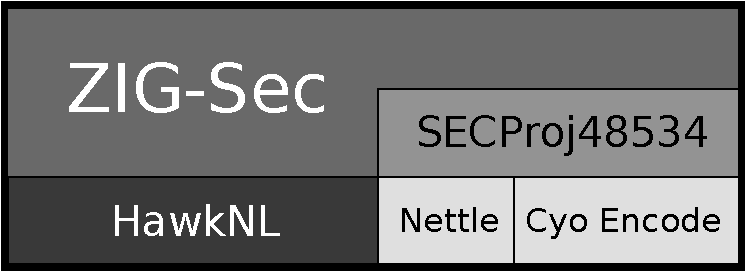
\includegraphics[width=0.7\linewidth]{images/security.pdf}
 \caption{Security module architecture} 
 \label{fig:security} 
\end{figure}

The module has been implemented by extending the ZIG library functionalities, providing secure communication, transparently to the application, being responsible for distributing cryptogaphic keys. It runs over HawkNL \cite{hawknl} and over SEC\ppse{}. HawkNL is a library that, among other functionalities, provides a simpler and portable API for sockets. SEC\ppse{} is our library that provides C++ abstractions for cryptographic algorithms available in Nettle \cite{nettle} and \mbox{CyoEncode} \cite{cyoencode}. SEC\ppse{} also implements certification and serialization functionalities meant for security related transmissions. Figure \ref{fig:security} illustrates the security module architecture.%Nettle is a low-level cryptographic library written in C, which offers algorithms for hashing (MD5, SHA1, SHA256 etc.), symmetric (AES, ARCFOUR, 3DES etc.) and assymetric (HMAC-MD5, HMAC-SHA-1 and HMAC-SHA-256) cryptography and generation of pseudo-random data (Yarrow). CyoEncode \cite{cyotec} is a small library which provides coding and decoding in Base64, Base32 and Base16.

In our secure communication protocol, all ZIG-generated packets sent, both by clients and by servers, are intercepted right before being transmitted through the network. In each one of them, a small header is introduced with control information used to guarantee confidentiality, integrity and authenticity of data when such attributes are required. The size of this header is variable, for it depends on what characteristics are desired by the application, and on the intended level of security (key length). For a real-time application, such as distributed games, usually there is no need for a very long key, because the hacker would have too little time to break the algorithm by brute force. For example, using AES and HMAC-MD5, it would be necessary only 21 bytes. In general, the overhead size of each packet is somewhere between 1 and 37 bytes. These packets containing user data and control header are then called \textbf{data packets}.

There is also another type of packet, called \textbf{control packet}, which is utilized to negotiate keys between peers who intend to communicate with each other. They are usually longer, for they need to attach a copy of the users certificates. However, these packets are sent only once in the beginning of the communication with a peer which has been unknown until that moment. Once they have negotiated a key, they only need to negotiate a new one when one of the peers loses it or if the key is already being used for a time long enough for the key to become breakable by brute force.

\begin{figure}[h]
  \centering 
  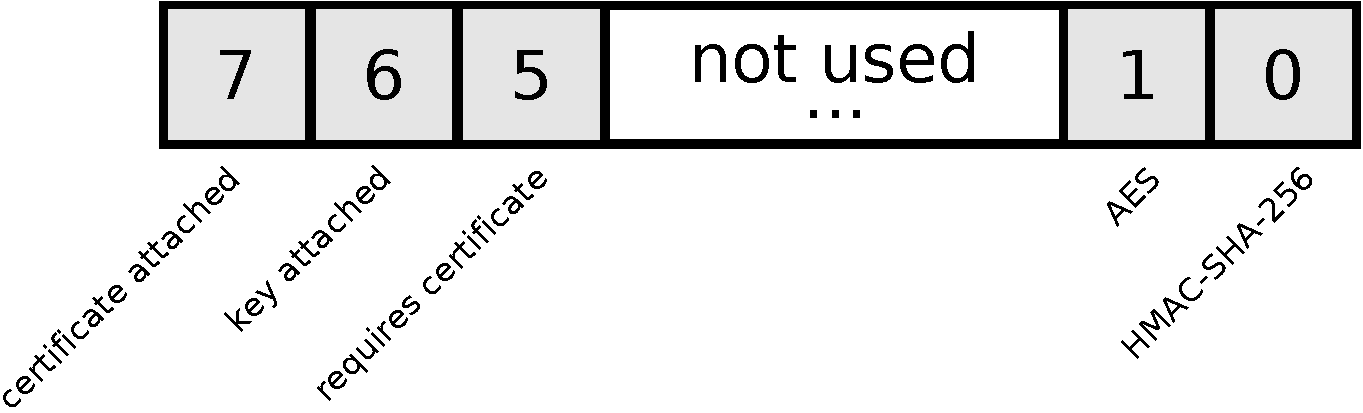
\includegraphics[width=1.0\linewidth]{images/header.pdf}
 \caption{Control header} 
 \label{fig:controlheader} 
\end{figure}

The control header consists of the packet descriptor (1 byte). As shown in Figure \ref{fig:controlheader}, the bit 0 indicates whether the data are protected by HMAC-SHA-256. The bit 1 indicates whether the data are encrypted with AES. Bit 5 indicates that the message source needs the destination host certificate. Bit 6 indicates that a key has been generated and attached to the packet in control data and bit 7 indicates that the certificate of the origin has been attached to the packet in control data. Bits 2, 3 and 4 are not used.

When the application requires the secure transmission of a packet to the security library, it must inform: data being transmitted, socket used for sending, address and port of the destination, type of desired security (confidentiality, authenticity and integrity) and the identification of the user which will receive the message at the provided address.

To guarantee confidentiality of the messages, it can be used both symmetric and asymmetric cryptographic algorithms. Both are considered secure, depending on the length of the key used. The secure communication protocol adopts the strategy of initially using an asymmetric cryptography algorithm to negotiate a key to be used then by each pair of computers to communicate securely with symmetric cryptography. This approach allows to reduce the processing time of encrypting and decrypting data, for symmetric cryptography requires less CPU time. Along with the confidentiality provided by this mechanism, authenticity may also be achieved by using hash functions with keys, also known as Message Authentication Code (MAC), to verify the authenticity and integrity of the messages.

Every time that a peer needs to communicate with another which was unknown until that time, they first need to negotiate a key. Therefore, before sending the data packet required by the application, the library sends a requisition for the certificate of the destination through a control packet, which already carries the source's own certificate. When the packet arrives in the destination peer, the security library reads the attached certificate and verifies its authenticity with  the specified certification authority responsible for the game. If the verification fails, the packet is discarded. If it succeeds, the process continues: the peer who received the packet allocates a reply packet, where it attaches its own certificate, as required, and a randomly generated key, which is encrypted using the public key present in the certificate of the peer that initiated the whole process. This way, it can be assured that only the receiver of this reply packet will be able to decrypt it and then obtain the key. To guarantee that the sender of this packet is not an attacker who intercepted the communication, the already encrypted key is re-encrypted, this time with the private key of the sender. This way, both authenticity and integrity are provided.

After receiving the reply packet containing the double-encrypted key, the first peer decrypts it using the public key of the other peer, verifying the authenticity of the message, and then decrypts it again, using  its own private key. When this whole process is successfully completed, the peers will be able to securely communicate with a fast symmetric cryptographic algorithm using the generated key.

\section{Simulations}
\label{sec:simulations}

Since one of the main objectives of the \ppse{} engine is to reduce the bandwidth utilization by the server, a numerical comparison between the load on a traditional server and the load on a \ppse{} server was required. In order to do that, it was necessary to simulate two game servers, each one with players connected to it. One of them was a traditional game server, to which the clients kept connected and trading packets the whole time. The other one was a \ppse{} server, where the players needed to trade packets with the server only while they were in the social space. In the action space, the players formed a peer-to-peer group, communicating to one another directly.

The ns-2 simulator \cite{mccanne:nsn} was used to create the simulated environment and perform the simulation itself. The servers and clients - both traditional and \ppse{} - were programmed extending the Application base class of the ns-2 API. The \ppse{} clients connect to the \ppse{} server, sending packets to it at a fixed rate while in the social space. The server, in turn, sends to each client in the social space an update containing information about all other clients in the same space. When a player leaves the social space and joins a peer-to-peer group of an action space, it stops exchanging packets with the server, due to its direct communication with the other players. The non-\ppse{} server and clients behave simply as follows: each client sends a packet to the server at a given fixed rate, while the server broadcasts an update to all clients, also at a fixed rate. Although this approach does not take into consideration possible optimizations on the server, such as interest management \cite{morse1996iml}, this is not relevant, since the same optimizations could be used in the social space of the \ppse{} server, resulting in a similar bandwidth usage reduction percentage, when comparing the two server models.

We based our simulation on some works, such as \cite{breu2007ogt}, \cite{park2005nta} and \cite{feng2005tcp}, which analyse the network traffic generated by action games, since this is the genre targeted by the \ppse{} engine. As in most first-person shooters, the transport layer protocol used was UDP. Each packet received by the server from the clients is 100 bytes long. The update sent to each client, containing information about all the players, is proportional to the number of players present in the game, for the traditional server. For the \ppse{} server, the update length is based only on the number of players in the social space. In both cases, the length of this update is 100 bytes multiplied by the number of players who will be updated. The interval between two consecutive packets received from each client is 150 ms, while the interval between two consecutive updates from the server to each client is 100 ms. Each player keeps alternating between the social space and the action space. The time he stays in each one of them is chosen randomly, ranging from 0 to 20 minutes, for each space change. The whole game session lasts for 1 hour.

\begin{figure}[h]
  \centering 
  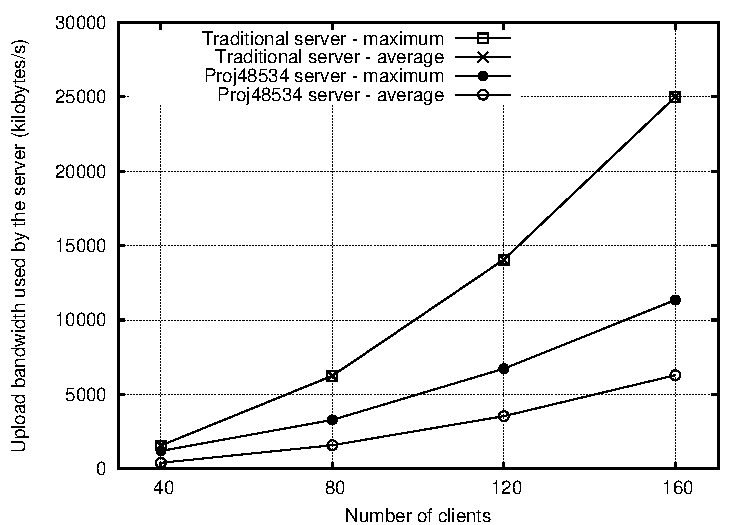
\includegraphics[width=1.0\linewidth]{images/upload_blinded.pdf}
 \caption{Upload bandwidth utilization by the server} 
 \label{fig:upload} 
\end{figure}

\begin{figure}[h] 
  \centering 
  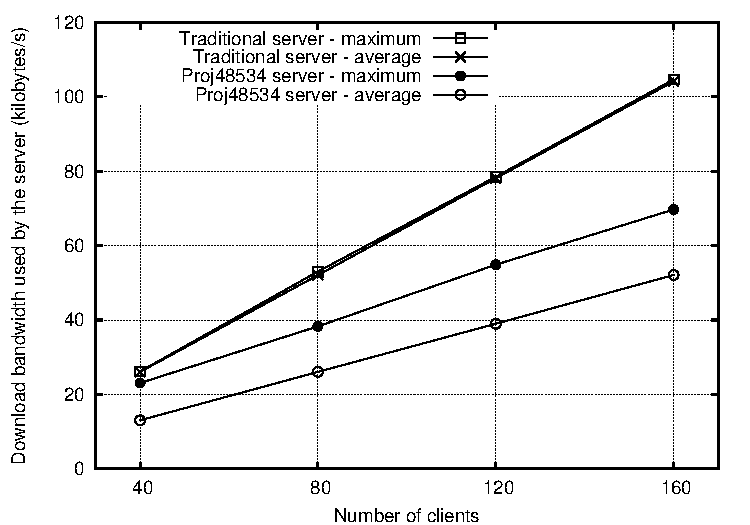
\includegraphics[width=1.0\linewidth]{images/download_blinded.pdf}
 \caption{Download bandwidth utilization by the server} 
 \label{fig:download} 
\end{figure}

The results were collected as follows: to measure the average upload bandwidth usage by the server, the sizes of all packets sent during the whole session were added up and then divided by the session time; to determine the maximum usage, it was measured how many bytes had been sent each second and the highest value was selected. In Figure \ref{fig:upload}, it is shown the maximum and average upload bandwidth utilization results found for a traditional server and a \ppse{} server. In Figure \ref{fig:download}, the download bandwidth usage is also depicted. Table \ref{tab:upload} and Table \ref{tab:download} show the numerical values of the average bandwidth utilization found in the simulation.

\begin{table}[h]
\caption{Average upload bandwidth utilization (kB/s)}
\centering
  \begin{tabular}{ c | c c }  
    \hline
    Clients & Traditional Server  & \ppse{} Server  \\ \hline
    40      & 1562.50             & 400.76          \\
    80      & 6250.00             & 1581.38         \\
    120     & 14062.49            & 3533.67         \\
    160     & 24999.98            & 6290.14         \\
  \hline
  \end{tabular}
\label{tab:upload}
\end{table}

\begin{table}[h]
\caption{Average download bandwidth utilization (kB/s)}
\centering
  \begin{tabular}{ c | c c }  
    \hline
    Clients & Traditional Server  & \ppse{} Server  \\ \hline
    40      & 26.04            & 13.02          \\
    80      & 52.08             & 26.04         \\
    120     & 78.12            & 39.00         \\
    160     & 104.17            & 52.09         \\
  \hline
  \end{tabular}
\label{tab:download}
\end{table}

As we can see, the average download bandwidth utilization is decreased by, approximately, one half, and the average upload bandwidth utilization is reduced to one quarter. This happens because the periods during which a client stays on the social and action spaces have approximately the same duration. In consequence of that, there are roughly half the clients exchanging packets with the server for each instant, in the average. As each client sends fixed size packets periodically to the server, the bandwidth occupation grows linearly, and so, as the number of players halves, so does the server's download bandwidth utilization. However, as the update sent by the server to each client is proportional to the number of clients being updated, the upload bandwidth utilization by the server grows quadratically. Therefore, when the number of players is divided by two, the upload bandwidth utilization of the server is divided by the square of two, that is, four.

It is important to notice, however, that the time a player usually spends playing action games, such as first-person shooters, is much longer than the time they keep talking in the game chat room. Therefore, the average time spent by each player in the social space should be much shorter than the time spent on the action spaces in the simulation. Also, the social space will most likely have much less need for frequent updates, allowing further decrease of the bandwidth utilization by the \ppse{} servers. Anyway, those parameters were chosen considering a pessimistic scenario, where the social space is as interactive as the action space, and the players spend more time socializing than it usually occurs in this kind of games.

\section{Conclusion}
\label{sec:conclusion}

We proposed a different approach to MMOGs, that uses P2P groups and transfers the simulation processing to them. In order to provide security and scalability, the game model was restrict to the instanced game model. The existence of a server-side  guarantees that, if deem necessary, the server can act as final arbiter. The performed simulations demonstrate that, even in a pessimistic scenario, the reduction of the average bandwidth usage by the game server can be significant. The download bandwidth utilization was reduced by one half, while the upload bandwidth utilization was the most benefited one, decreasing by 75\%, allowing to reduce the maintenance cost of such kind of server.

We are currently integrating the \ppse{} architecture with our game prototype, \hoverkill{}. This game is a client-server capture-the-flag tank game, and its network system is being replaced by our architecture. The final goal is to be able to test the game in client-server and peer-to-peer modes, in order to base our conclusions in real results rather than simulations.

\section*{Acknowledgements}
\label{sec:ack}

This work was supported by the Funding for Studies and Projects (FINEP), %through the \ppse{} project (\ppse{}-5849-1),
and by the National Research Council (CNPq).

% \begin{figure} 
%   \centering 
%   
\includegraphics[width=0.8\linewidth]{example.pdf}
%  \caption{Example of image} 
%  \label{fig:example} 
% \end{figure}

\bibliographystyle{sbgames}
\bibliography{ppsg}
\end{document}
